\renewcommand{\theequation}{\theenumi}
\begin{enumerate}[label=\thesection.\arabic*.,ref=\thesection.\theenumi]
\numberwithin{equation}{enumi}
\item The figure for A quadrilateral obtained in the question looks like Fig. \ref{fig:quad}.
with side $a$, $c$, $e$ and $d$.
\\
%\renewcommand{\thefigure}{\theenumi.\arabic{figure}}
\begin{figure}[!ht]
\centering
\resizebox{\columnwidth}{!}{\input{./figs/quadrilateral.tex}}
\caption{Quadrilateral ABCE by Latex-Tikz}
\label{fig:quad}	
\end{figure}
%
%
%\renewcommand{\thefigure}{\theenumi}
%
\item List the design parameters for construction
\label{const:table1}
\\
\solution See Table. \ref{table:table1}. 
%
\begin{table}[ht!]
\centering
\input{./tables/inp.tex}
\caption{To construct quadrilaterl $ABCE$}
\label{table:table1}	
\end{table}
\item Find the coordinates of the various points in Fig. \ref{fig:quad}
\label{const:quad}
\\
%
\solution From the given information, 
\begin{align}
\label{eq:constr_a}
\vec{A} &= \myvec{p\\q} 
\\
\vec{B} &= \myvec{0\\0}, 
\label{eq:constr_b}
\\
\vec{C} &= \myvec{c\\0}
\label{eq:constr_c}
\\
\vec{D} &= \myvec{b\\0}
\label{eq:constr_d}
\\
\vec{E} &= \myvec{r\\s}
\label{eq:constr_e}
\end{align}

\textbf{For Vertices A}
\\
\begin{equation} \label{eq:one}
AB={\Vert A-B \Vert}^2={\Vert A\Vert}^2=a^2
\end{equation}

\begin{equation}
DB={\Vert D-B \Vert}^2={\Vert D\Vert}^2=b^2
\end{equation}

\begin{equation} \label{eq:two}
AD={\Vert A-D \Vert}^2=a^2
\end{equation}
\\
Solving equation \ref{eq:two}\\
$a^2=A^TA+D^TD-A^TD-D^TA$\\
$a^2={\Vert A\Vert}^2+{\Vert D\Vert}^2-2A^TD$\\
$a^2=a^2+b^2-2pb$\\
\begin{equation}
p=\frac{b^2+a^2-a^2}{2b}=\frac{b^2}{2b}=\frac{b}{2}
\end{equation}
\\
From equation \ref{eq:one}
\\
$\Vert A \Vert =a^2= p^2+q^2$\\
\begin{equation}
q=\pm \sqrt{a^2-p^2}
\end{equation}
\\
\textbf{For Vertices E}\\
If we draw perpendicular line from E, it meets on x-axis at point O.\\
Consider $OC =g$
Then, 
\begin{equation}
cos \theta _1 = \frac{OC}{EC}=\frac{g}{e}
\end{equation}

\begin{equation}
g = e cos\theta _1
\end{equation}
\begin{equation}
tan\theta _1=\frac{OE}{OC}=\frac{h}{g}
\end{equation}

\begin{equation}
h=gtan \theta _1
\end{equation}

\begin{equation}
r = c+g
\end{equation}
\begin{equation}
s = h
\end{equation}

The values are listed in 
%\item List the  derived values.
%\label{const:table2}
%\\
%\solution See  
Table. \ref{table:table2} 
\begin{table}[ht!]
\centering
\begin{tabular}{ |p{3cm}|p{3cm}|  }
\hline
 \multicolumn{2}{|c|}{Derived Values.} \\
\hline
$\vec{A}$ & $$\begin{pmatrix}1.5\\2.6\end{pmatrix}$$\\					
\hline
$\vec{C}$ & $$\begin{pmatrix}4.1\\0\end{pmatrix} $$\\
\hline
$\vec{E}$ & $$\begin{pmatrix}5.05\\3.55\end{pmatrix} $$\\
\hline
\end{tabular}
\caption{To construct $ABCE$}
\label{table:table2}
\end{table}
%
\item Draw Fig. \ref{fig:quad}.	
\\
\solution The  following Python code generates Fig. \ref{fig:quad}
%
\begin{lstlisting}
codes/quadrilateral.py
\end{lstlisting}
\begin{figure}[!ht]
\centering
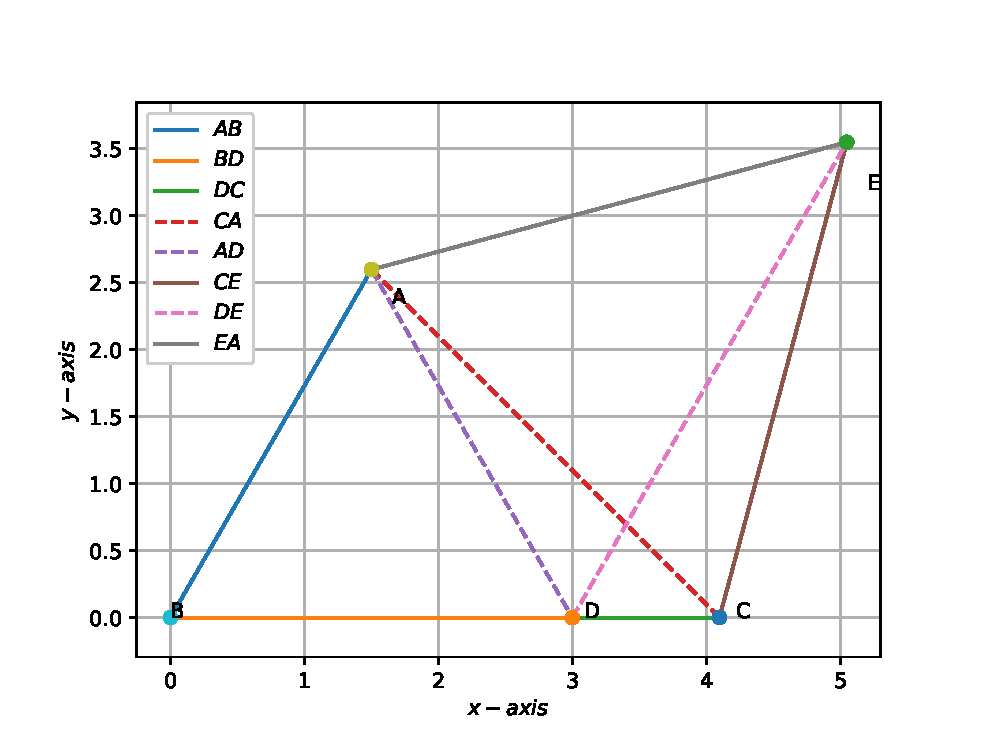
\includegraphics[width=\columnwidth]{./figs/quadrilateral.eps}
\caption{Quadrilateral generated using python}
\label{fig:quad_py}
\end{figure}

%
and the equivalent latex-tikz code generating Fig. \ref{fig:quad_py} is 
\begin{lstlisting}
figs/quadrilateral.tex
\end{lstlisting}
%
The above latex code can be compiled as a standalone document as
\begin{lstlisting}
figs/quadrilateral_fig.tex
\end{lstlisting}

\end{enumerate}

